\section{Le build}\label{section_build}

La tâche de \textit{build} concerne un processus automatisé qui permet de réaliser des opérations de compilation et de déploiement pour construire par exemple les versions distribuées par Smartesting à ses clients.
Ce processus a été modifié afin de pouvoir fragmenter les plugins existants.

\subparagraph*{}
Au début du stage, le \textit{build} permettait de déployer deux plugins pour les deux modeleurs RSM et Together.
L'objectif fut donc d'entreprendre la modification de celui-ci pour faciliter la création et le déploiement d'autres plugins, en vue de progressivement passer des modules Java en plugins pour Eclipse.

\begin{figure}[!h]
\begin{center}
  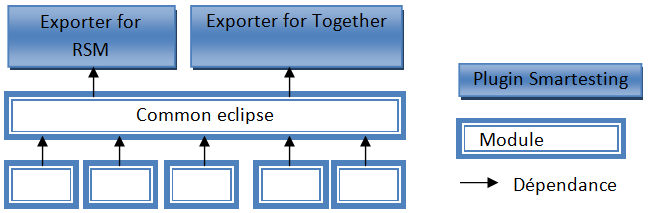
\includegraphics[scale=.6]{images/AvantBuild.png}
  \caption{Projet avant amélioration du \build}
  \label{AvantAmeliorationBuild}
\end{center}
\end{figure}
\ \\
Sur la figure \ref{AvantAmeliorationBuild} p.\pageref{AvantAmeliorationBuild}, les modules de type plugin sont gérés spécifiquement pour être déployés via un ``update-site''.

\subsection{Objectifs}

L'un des objectifs de l'amélioration du \build est de pouvoir créer des plugins Eclipse et les déployer.
La stratégie doit permettre de différencier plusieurs types de modules :
\begin{itemize}
  \item Update-site
  \item Feature
  \item Plugin (Smartesting)
  \item Module Java
  \item Librairie Java
  \item Plugin Eclipse
\end{itemize}
\ \\
La figure \ref{AmeliorationBuild} p.\pageref{AmeliorationBuild} montre l'amélioration apportée au \build. 
On peut remarquer la diversité des types de modules et des relations de dépendance.
La gestion des dépendances qui est aussi un enjeu puisqu'il faut que le \build construise les fichiers de configuration des plugins.

\begin{figure}[!h]
\begin{center}
  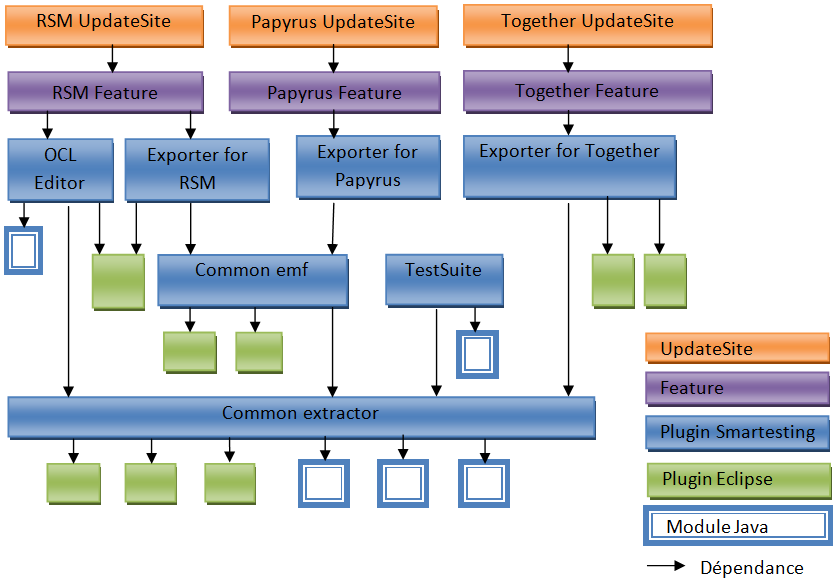
\includegraphics[height=7.5cm]{images/AmeliorationBuild.png}
  \caption{Projet après amélioration du \build}
  \label{AmeliorationBuild}
\end{center}
\end{figure}

\subsection{Fonctionnement du \build}

Le développement de la solution Smartesting est réalisé grâce à l'éditeur Java, IntelliJ\footnote{IntelliJ ou IDEA} de JBrain.
Il s'agit d'un éditeur payant dont le fonctionnement est proche de l'éditeur Java fonctionnant sous Eclipse.
Cet éditeur offre de nombreuses fonctionnalités qui rendent le développement plus facile.

\subparagraph*{}
Le \build mis en place par Smartesting, utilise les fichiers d'IntelliJ pour gérer les dépendances entre les modules.
Il y a donc une tâche \textit{ant} qui a été développée par Smartesting pour réaliser cela.

\subsubsection{Génération du manifest :}

La génération du manifest du plugin a été effectuée à partir d'un fichier manifest maintenu par le programmeur. 
Il est situé dans les sources du module plugin d'IntelliJ.
On y trouve la description du plugin et certains paramètres.
A l'intérieur de ce fichier, la version, le nom et les librairies Java sont générés automatiquement.

Exemple :
\tiny
\begin{verbatim}
Manifest-Version: 1.0
Bundle-ManifestVersion: 2
Bundle-Name: Exporter Plug-in
Bundle-SymbolicName: @plugin.identifier@;singleton:=true
Bundle-Version: @plugin.version@
Bundle-Vendor: SMARTESTING
Bundle-RequiredExecutionEnvironment: J2SE-1.5,
 JavaSE-1.6
Bundle-Classpath: .@plugin.runtime.manifest@
Require-Bundle: com.ibm.xtools.modeler;visibility:=reexport,
 com.ibm.xtools.modeler.ui;visibility:=reexport,
 \ldots
 com.smartesting.eclipse.emf;visibility:=reexport,
 com.smartesting.testsuite
Bundle-Activator: com.smartesting.ltd.eclipse.common.plugin.SmartestingPlugin
Bundle-Localization: plugin
Bundle-ActivationPolicy: lazy
Export-Package: com.smartesting.ltd.eclipse.rsm7.testsuite,
 com.smartesting.ltd.eclipse.rsm7.translator.extractor
\end{verbatim}
\normalsize

Dans cette exemple on y retrouve encadré par les @ les informations générées automatiquement.
Les autres informations sont spécifiques à chaque plugin.

\subparagraph*{}
Résultat de la génération :
\tiny
\begin{verbatim}
Manifest-Version: 1.0
Bundle-ManifestVersion: 2
Bundle-Name: Exporter Plug-in
Bundle-SymbolicName: com.smartesting.rsm.exporter;singleton:=true
Bundle-Version: 1.0.0.44657
Bundle-Vendor: SMARTESTING
Bundle-RequiredExecutionEnvironment: J2SE-1.5,
 JavaSE-1.6
Bundle-Classpath: .,
 lib/commons-lang-2.3.jar
Require-Bundle: com.ibm.xtools.modeler;visibility:=reexport,
 com.ibm.xtools.modeler.ui;visibility:=reexport,
 \ldots
 com.smartesting.eclipse.emf;visibility:=reexport,
 com.smartesting.testsuite
Bundle-Activator: com.smartesting.ltd.eclipse.common.plugin.SmartestingPlugin
Bundle-Localization: plugin
Bundle-ActivationPolicy: lazy
Export-Package: com.smartesting.ltd.eclipse.rsm7.testsuite,
 com.smartesting.ltd.eclipse.rsm7.translator.extractor
\end{verbatim}
\normalsize
